\pagenumbering{arabic}
\chapter{Project Proposal}

\section{What’s the potential for this project?}

Climate change is already beginning to affect global systems beyond the observed average annual temperature rises \cite{ipcc2021},\cite{nrdc2023effects}.
    Net Zero means taking necessary actions to install systems which are designed to ensure “any emissions would be balanced by schemes to offset an equivalent amount of green house gases (GHG) from the atmosphere”
\cite{ukgov2023}.

This complex problem has multiple facets, however one approach is to triage the source of GHG contributions, for example:
\\
To produce 1000 tons of steel, up to 1850 tons of CO2 is produced \cite{mckinsey2020decarbonization}. 
In 2019, 1.875 Billion tons of steel was produced. This means that at least 3.375 billion tons of CO2 was produced. 37 Billion metric tons represents the global GHG emissions in both 2019 \& 2022 (2020: 35 Billion) \cite{hausfather2022global}. 65\% of emissions is attributable to CO2 and fossil fuel \cite{Jones2023CO2}.
\\
\\
Waste heat recovery systems represent a significant environmental opportunity, and one that is economically aligned with industry. Waste heat reclamation would reduce operational costs and energy consumption in steel manufacture alone by 45\% \cite{doe2008wasteheat}. 
\\
This project plan outlines a path for systematic search and demonstration of value-accretive metasurfaces suitable for such renewable energy settings, namely photovoltaics.

To date, all but one commercial thermo-photovoltaic (TPV) system has been built (by JX Crystals) - based on an emitter material composite designed to be ``well-matched'' for Gallium Antimonide (GaSb) cells \cite{ferguson_matched_1997}, \cite{fraas2002thermophotovoltaics}. However, Antora energy is soon expected to begin production after a 40\% efficient TPV system was demonstrated - an important threshold for being comparable to steam-driven turbines \cite{thermophotovoltaic2022efficiency}, \cite{pv_magazine_2023_thermophotovoltaic}. With no moving parts, and high theoretical efficiency ceiling, TPV is a promising candidate for the next wave of engineering effort to carefully consider, with still considerable headroom for improvement.
\\
On the other hand, the installed base of solar photovoltaics already (as of 2022) exceeds 1.185 Terrawatts, accounting for 6\% of global needs (up from 3\% in 2019) \cite{ieapvps2023}, \cite{ieapvps2020}. This technology is not without downsides; ways to improve efficiency and reduce environmental cost must be found.

Research impact for this project will follow from answers to the intriguing questions posed. What unique sensing, detection, and energy harvesting capabilities exist? Is `dynamic' tunability required? Can the design of metasurfaces be systematically customised to achieve desired absorption responses at specific frequency ranges? The unifying theme: is it viable to design manufacturable metasurface architectures that enhance photovoltaic systems?


\section{Background}

Theoretical ‘Metamaterials’ were suggested in the 1960s, but it was unknown how practical realisation could be accomplished \cite{veselago1968}. By the mid-1990s it was realised geometric features, rather than chemical composition alone, could be utilised to architect the response of incident waves (Guo2023 \cite{Guo2023}). Collaboration between Imperial College London and the Marconi Company revealed that, within the realm stealth technology, the geometric contribution of thin carbon fibres significantly influenced the structure's electromagnetic response; more so than the underlying characteristic properties of the material itself. Meta simply means to `go beyond’ naturally-occurring materials.

Experimental exhibition of a metamaterial with induced negative index of refraction was achieved shortly after; simultaneously negative electric and magnetic responses within a composite of non-magnetic materials (Smith2000 \cite{smith2000}, \cite{shelby2001}).
Metasurfaces (two-dimensional equivalents), have recently been used to demonstrate seismic cloaking (earthquake prevention) by controlling surface waves on the earth \cite{palermo2018}.
Given the complexity of attaining Net Zero there was never a more pertinent time to access the viability of metasurface designs.
In the realm of energy-harvesting, metamaterials have been engineered with perfect absorptance; transmission and reflection may be suppressed entirely. At the same time, they possess excellent characteristics that can break the thickness limitation of traditional bulky absorption devices. A comprehensive and up-to-date overview of meta-absorber achievements may be readily found (Wang2023) \cite{wang2023broadband}.

\begin{figure} [!h]
	\centering
	%\captionsetup{justification=centering}
	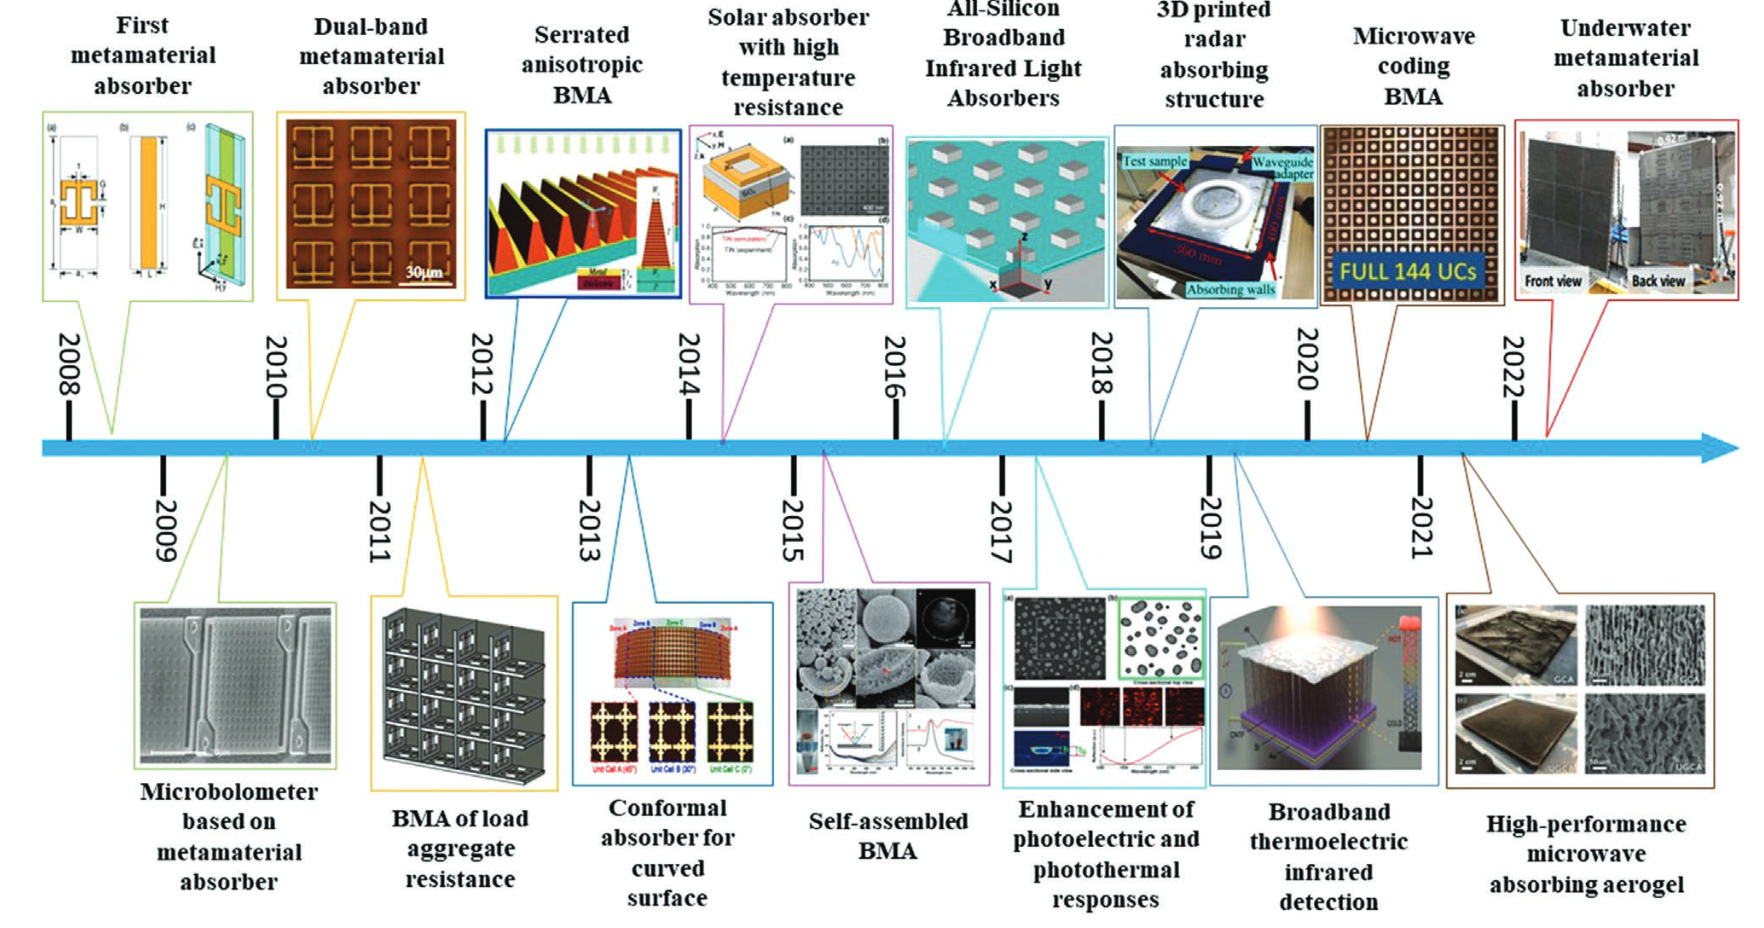
\includegraphics[width=14cm,height=8cm,keepaspectratio]{figures/introduction/achievements}
	\setlength\belowcaptionskip{3pt}
	\caption{Achievements to date in metamaterial absorbers \cite{wang2023broadband}}
	\label{some-figure}
\end{figure}

This resource highlights the necessity for a deeper exploration. This project will focus on the design, functionality, and application of these materials. Wang2023 underscores the importance of developing multifunctional absorption devices, capable of integrating various applications such as energy harvesting, photodetectors, stealth technology. This project will focus on opportunities for tunable and reconfigurable metamaterials that adapt to environmental changes - thereby enhancing the performance and scope of these absorbers.

\begin{figure} [!h]
	\centering
	%\captionsetup{justification=centering}
	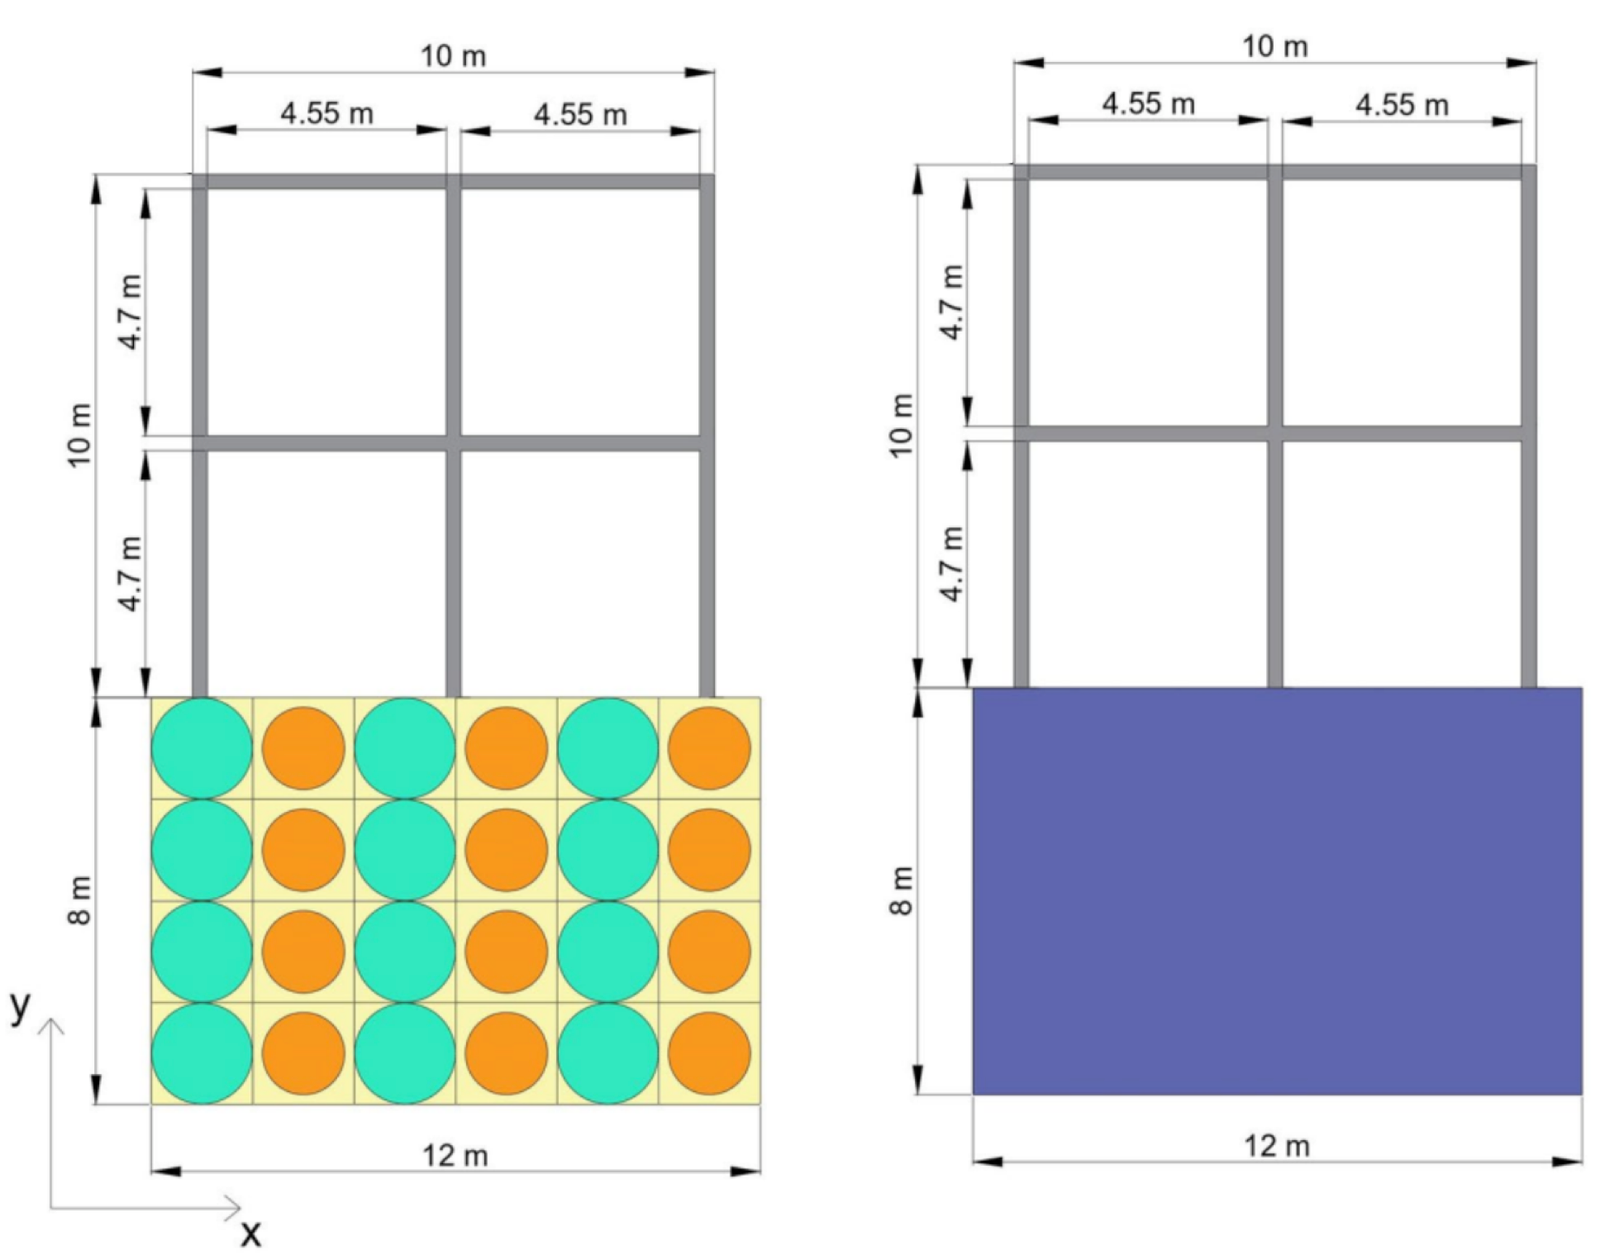
\includegraphics[width=14cm,height=8cm,keepaspectratio]{figures/introduction/cloak.png}
	\setlength\belowcaptionskip{3pt}
	\caption{Illustrating the potential of metamaterials: Steel frame on metamaterial foundation (a),  concrete foundation (b). (Gupta2023 \cite{Gupta2023}). }
	\label{some-figure}
\end{figure}









% Here the Equation \ref{reaction-oxidation-sto} starts:
% \begin{equation}
% 	k \cdot \ce{ SrTiO3} \ce{->} p \cdot \ce{ SrTiO3}  +   q \cdot \ce{SrO (SrTiO3)_n} +  q \cdot \ce{TiO2},
% 	\label{reaction-oxidation-sto}
% \end{equation}
% where $k = q\cdot (n+1) + p$. And here it ends.
%  We are in the Section \ref{section-with-figure} with Figure \ref{some-figure}.



\section{Aims and Objectives} \label{section-with-figure}

Due to unit cell size varying inversely with the resulting resonant frequency value, the focus will be on producing a holistic framework for Metasurface design, to ensure the platform has compatibility with a variety of target devices.
% semiconductors across the electromagnetic spectrum

The focus of designs that adapt to environmental changes and requirement of specialist equipment required for nanometer structures shall prompt experimental work to begin in lower frequency ranges with the intention of moving onto higher frequency regimes:

\begin{table}[h]
\centering
\begin{tabular}{|l|l|l|}
\hline
\textbf{Frequency Regime} & \textbf{Wavelength Range} & \textbf{Frequency Range} \\ \hline
L-Band to S-/C- Band & 30cm to 6cm & 1 GHz to 5 GHz \\ \hline
Microwave to Mid Infrared & 1mm to 1 $\mu$m & 300 GHz to 300 THz \\ \hline
Far Infrared to Visible & 100$\mu$m to 380nm & 3 THz to 790 THz  \\ \hline
\end{tabular}
\caption{Summary of Frequency Regimes for project milestones}
\label{tab:frequency_regimes}
\end{table}


To accelerate experimental validation, within Year 1 work will begin on physically larger Surface Acoustic Wave (SAW) devices (millimetres to centimetres). The influence of environment - ice, humidity, dirt and contaminants - shall be feasibly studied at this scale for how they alter metasurface absorption profiles. It is essential to understand and how these factors will play a role in real-world [thermo]photovoltaic applications - since coupling modes would be confounded by environmental factors, most likely. When resonator devices `couple' there are emergent resonant modes. Coupling by Surface Acoustic Waves not only modulates resonator eigenfrequencies (dispersive coupling) but also their damping (dissipative coupling) \cite{Rieger2022SurfaceAW}. Metasurface designs that are `optimised' would yield specific absorptivity and emissivity characteristics, in this instance, for efficient energy harvesting and/or sensing at and around these frequencies. 

% This is wehere the environmental sensing will be demonstrated. Instead of framing this around a collaboration with on-going research, it is better to link this with environmental sensing for (thermo)photovoltaics. Is it humidity, icing, contamination, dirt, combination of these etc.. that will be sensed? If so, what will be designed/optimised? How it will be tested/characterised?


\section*{L-Band (Year 0.5 to 1.5):}
\begin{itemize}
    \item Objective 1: Sense environment changes, with a focus on water and ice.
    \begin{itemize}
        \item Utilise resonance response in the presence of droplets, ice crystals and piezoelectric acoustic waves.
    \end{itemize}
    \item Objective 2: Measurement and detection of ice cracks.
    \begin{itemize}
        \item Draw parallels between photovoltaic defect detection.
    \end{itemize}
    \item Aim: Develop a holistic design framework to equip a multi-functional [MM-SAW] device with sensing capability.
\end{itemize}

\section*{Microwave to Infrared (Year 1 to 2.5):}
\begin{itemize}
    \item Objective 1:
     Maximize thermal emission in the atmospheric window to radiate heat away.
    \begin{itemize}
    \item Advanced materials designed for passive radiative cooling can radiate heat directly into the coldness of space through an infrared range where the atmosphere is transparent to thermal radiation \cite{Rephaeli2014RadiativeCooling}.
    \end{itemize}
    \item Objective 2: Implement active thermal capture for thermoelectric conversion through photon recycling.
    \item Aim: Expand the framework - design, fabrication, characterisation.
\end{itemize}

\section*{Infrared to Visible (Year 2.5 to 3):}
\begin{itemize}
    \item Objective 1: Simulate enhanced photovoltaic efficiency through enhanced light absorption, amorphous silicon is a suitable device-coupling-candidate.
    \item Objective 2: Investigate feasibility of enhanced efficiency through light capture and (non-lossy) frequency conversion processes i.e. SHG.
    \item Aim: Expand the framework - exploration and design.
\end{itemize}
\vspace{5mm}
Deep Learning methods for the objective of parameter search through inverse design is emerging as a viable alternative to traditional Particle-In-Cell-Simulations \cite{Nadell2019}. In the context of thermophotovoltaic systems this would relate to designing refractory metamaterials capable of surviving high radiator temperatures while attaining suitably (low) emitter frequencies, to match the photovoltaic bandgap (Coutts1999 \cite{coutts1999}).
\begin{figure} [!h]
	\centering
	%\captionsetup{justification=centering}
	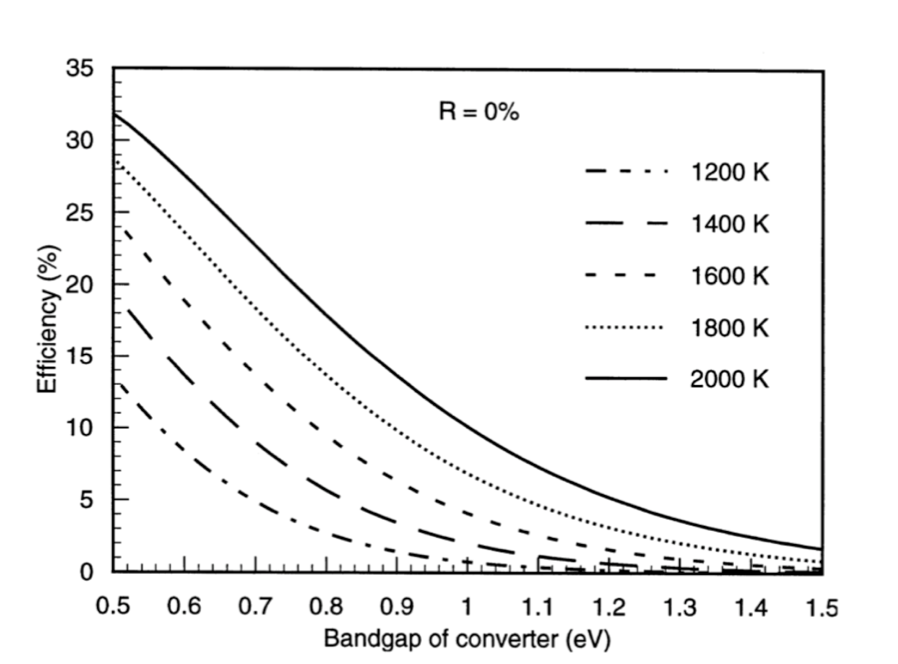
\includegraphics[width=14cm,height=8cm,keepaspectratio]{figures/introduction/tpv1.png}
	\setlength\belowcaptionskip{3pt}
	\caption{Modelled variation of efficiency with bandgap of the converter. The radiator temperature is treated parametrically. No sub-bandgap photons are returned to the radiator (Coutts1999 \cite{coutts1999})}
	\label{some-figure}
\end{figure}

In Year 2 individual lab-scale demonstrations will begin, with an emphasis on performant designs for mission-critical aspects of the thermophotovoltaic system; photon recycling, higher radiator temperatures, and targeted bandgap-matching.
Building on the environmental sensing achievements in Year 1, there shall be a consideration for necessary and achievable value-adding sensing or detection capabilities within the context of envisioned operational settings for [thermo]photovoltaic systems. The focus will be to identify sensing capabilities that are synergistic and can be readily integrated via absorption tuning. For example, carbon auditing.
% , particulate presence, or pollutant concentrations. 

One envisioned setting for thermophotovoltaics is industrial steel manufacture. Carbon auditing would relate to the varying rate of waste heat recycling. It may prove useful to account this for auditing purposes.
% Particulate composition is also of interest, since air quality is a growing concern \cite{sokhi2022advances}. Constituent material choices for metamaterial composites are themselves subject to changes in temperature, voltage, pump light, and thus may be considered ‘active’ \cite{wang2023broadband}. Through thermally-induced phase changes between amorphous/crystalline states of their chosen substrate, Patel2021 were able to measure concentration differences in haemoglobin via refractive index measurements - using precisely tuned shifts in the absorption spectrum over a reference range of wavelengths \cite{Patel2021}. This mechanism, and others, shall be investigated for airborne particle concentrations. Existing detection methods for the seven green house gases would be reviewed. For instance, the criteria of ‘dangerous’ oxidant levels in the atmosphere is a reading above 0.15 ppm measured within 1 hour and involves manually-operated equipment \cite{manahan_environmental_chemistry}; pollutant levels in many locations is very likely undermonitored.
\\
In Year 2.5 to 3 attention shall be paid to commercial fabrication techniques. One ‘roll-to-roll’ polymer-based metasurface has been identified \cite{Ma2023}. The author reinforces the potential for ‘trench-like’ structures to be redesigned with active thermal management - a statement that echoes the research gap being addressed in this proposal.

        The primary question for scaled-up production is whether to recommend “Industry 4.0” or traditional manufacturing. Foundries vary widely in production volumes \cite{wiki:memsfoundries}; high volumes may infer low cost per unit albeit at high overhead. Alternatively, additive manufacturing unlocks ‘mass customisation’. This consideration may become crucial for market adoption at flexible production volumes.


\section{Indicative Methodology}


\subsection{Literature Review}
\begin{itemize}
    \item Review literature on Metasurfaces, thermophotovoltaic systems, and environment sensing.
    \item Analyse relevant Machine Learning methods for parameter search in Metasurface design.
\end{itemize}

\subsection{Simulation and Modeling}
\begin{itemize}
    \item Utilise simulation software to model and simulate proposed designs.
    \item Where possible validate simulations using data from real experiments or values obtained from published literature.
    \item Establish a comprehensive understanding of solver operations in simulation software and physical models.
\end{itemize}


\subsection{Experimental Validation}
\begin{itemize}
    \item Align with ongoing research efforts at Smart Materials \& Surfaces Lab to begin experiments.
    \item Progressively work towards experiments at higher frequencies.
\end{itemize}

\subsection{Environmental Sensing Development}
\begin{itemize}
    \item Develop algorithms for sensing, considering real-world scenarios.
\end{itemize}

\subsection{Collaboration \& Characterisation}
\begin{itemize}
    \item Collaborate with expert researchers to gain access and training on specialist lab equipment (e.g. new SHG capabilities expected in Durham by Autumn 2024)
\end{itemize}

\subsection{Application of Metasurface Framework}
\begin{itemize}
    \item Design architectures for specific frequency regimes, focusing on environment sensing, defect detection, absorption, passive cooling, and thermal energy conversion.
\end{itemize}

\subsection{Lab-Scale Fabrication}
\begin{itemize}
    \item Initiate lab-scale demonstrations, tailoring the metasurface platform to elements that contribute significantly to TPV system efficiency.
\end{itemize}

\subsection{Commercial Fabrication Consideration}
\begin{itemize}
    \item Evaluate viable manufacturing techniques, for consideration of routes to market.
\end{itemize}



\section{Research Plan}


\begin{figure}[h]
    \centering
    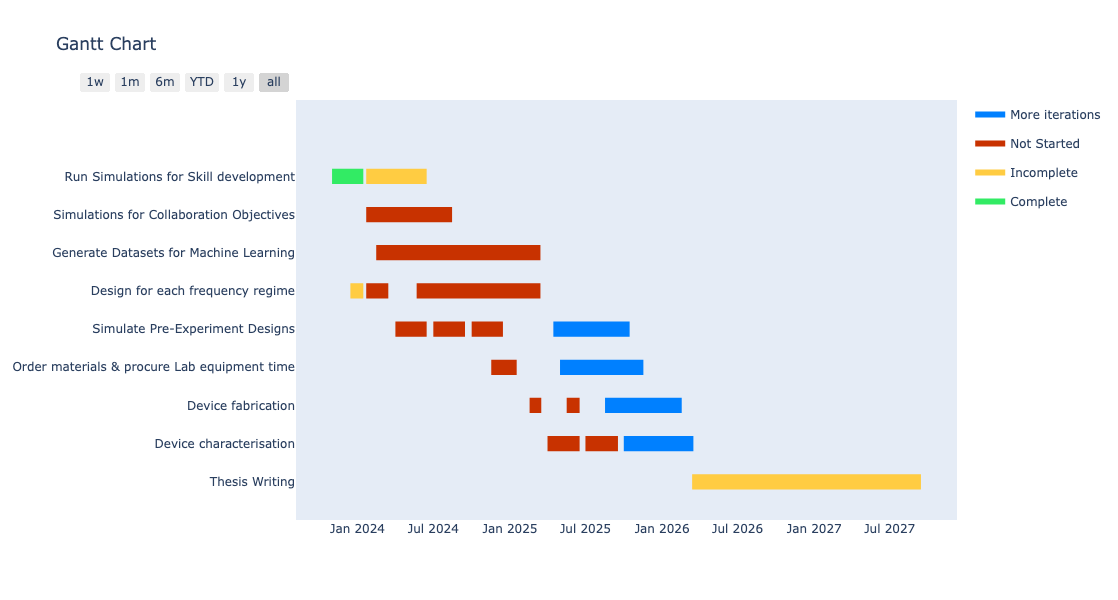
\includegraphics[width=\textwidth]{figures/introduction/gantt.png}
    \caption{Gantt Chart}
    \label{fig:your_label}
\end{figure}


\begin{sidewaysfigure}
    \centering
    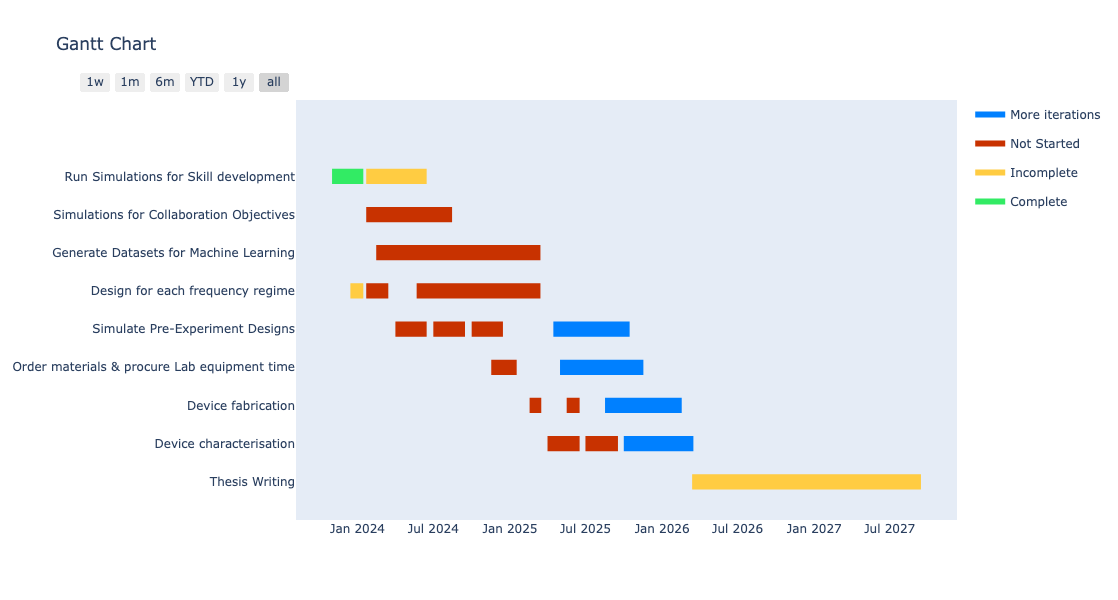
\includegraphics[width=\textwidth]{figures/introduction/gantt.png}
    \caption{Gantt Chart}
    \label{fig:your_label}
\end{sidewaysfigure}